\begin{flushleft}
 {\footnotesize{ \textsl {An intellect which at a certain moment would know all forces that set nature in motion, and all positions of all items of which nature is composed, if this intellect were also vast enough to submit these data to analysis, it would embrace in a single formula the movements of the greatest bodies of the universe and those of the tiniest atom; for such an intellect nothing would be uncertain and the future just like the past would be present before its eyes.}}} \\
\footnotesize  Pierre Simon Laplace, A Philosophical Essay on Probabilities\\
\end{flushleft}

En este capítulo se discutirán los resultados obtenidos a lo largo del trabajo. Está dividido en dos secciones, la primera está dedicada a recintos con una única puerta y la segunda a recintos con dos puertas sobre la misma pared.  

\section{Una puerta}

En esta sección se compararán los campos de presión y velocidad para recintos con puerta ancha (3,6~m) y angosta (1,2~m). También se hará una comparación de la presión y velocidad en función del tiempo que poseé un individuo que comieza en el medio de la habitacón.    

\subsubsection{Puerta ancha (3,6~m)}

Los resultados que se presentan en esta subsección son de simulaciones hechas para un recinto de  $20\times 20$~(m) con 225 individuos y una puerta centrada en la posición $x=20$~m e $y=10$~m con un ancho $L=3,6$~m.\\
En la figura \ref{isobaras_flujo_3_6m} (izquierda) se muestra un gráfico de isobaras. Puede verse que la zona de mayor presión se da a los costados de la puerta mientras que en el medio la presión es menor (sobre todo en la zona más proxima a la puerta). La distribución de presiones es simétrica con respecto al eje $y=10~m$. 

\begin{figure}[H]
    \centering
    \includegraphics[scale=1]{figuras/press_225p_v4_onedoor_3_6.eps}
        \includegraphics[scale=1]{figuras/flujo_door_3_6m.eps}
    \caption[width=5cm]{Izquierda: Isobaras cercanas a la puerta; la escala a la derecha está expresada en [PV]=N.m. Derecha: Gráfico de flujo de velocidad. Para ambos gráficos, la salida está centrada en la posición $x=20$~m e $y=10$~m y tiene ancho $L=3,6$~m. El recinto es de $20\times 20$~(m) con 225 individuos. La gráfica corresponde a valores medios a lo largo de 30 procesos de evacuación. Se usó un grillado de 1m$^2$ para promediar los campos de presiones y velocidad. La velocidad deseada de los individuos fue de $v_d=4$~m/s.}
    \label{isobaras_flujo_3_6m}
\end{figure}

El gráfico de la derecha muestra el promedio del flujo de velocidades. El ancho del trazo denota la magnitud del módulo de la velocidad. La mayor celeridad se obtiene en la zona del medio (en la coordenada y), dando a entender que los individuos que se encuentran en dicha región evacúan más rapido que los indvididuos que van por los costados. 
Puede verse que las zonas de alta presión coinciden con zonas de baja velocidad (costados) mientras que las zonas de alta velocidad son áreas con menor presión (centro). 

La relación entre presión y velocidad se condice con los resultados obtenidos en la figura \ref{pv_vel_t_100_3_6}. Allí se muestran la presión y velocidad en función del tiempo para un individuo que comienza en el medio de la habitación ($x=12,35$~m e $y=8,45$~m). Al principio su velocidad aumenta sin que la presión se vea afectada ya que corre hacia la salida sin interactuar con el resto de los peatones. Luego, su velocidad disminuye conforme su presión incrementa. En este momento la salida se obstruye y la multitud se amontona. Finalmente la velocidad vuelve a aumentar y su presión disminuye, en este momento el individuo logra hacerse paso para evacuar. 

\begin{figure}[H]
    \centering
    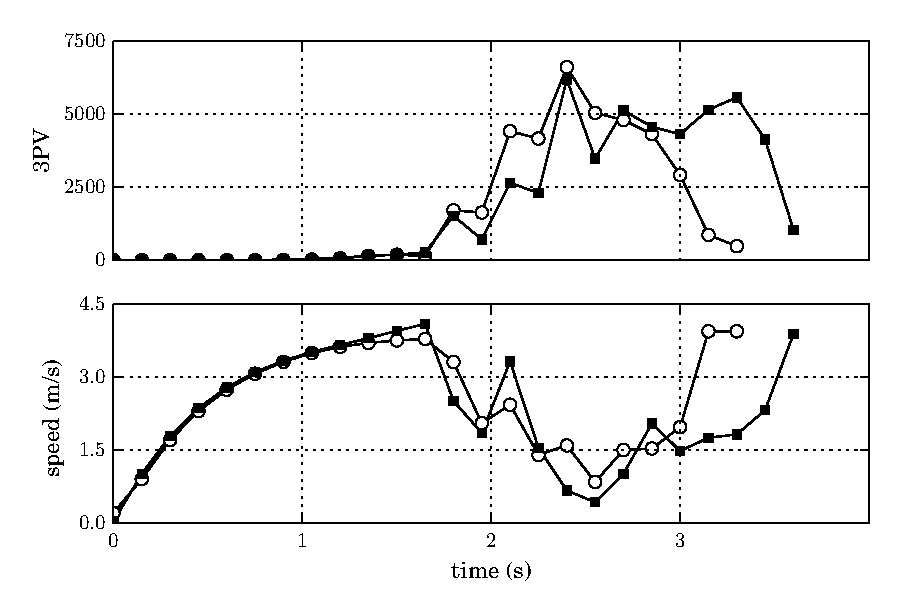
\includegraphics[scale=0.8]{figuras/pv_vel_t_100_3_6.eps}
    \caption[width=5cm]{Gráfico de velocidad(inferior) y presión(superior) en función del tiempo para un individuo ubicado inicialmente en $x=12,35$~m e $y=8,45$~m.  La salida está centrada en la posición $x=20$~m e $y=10$~m y tiene ancho $L=3,6$~m. El recinto es de $20\times 20$~(m) con 225 individuos. La gráfica corresponde a dos iteraciones diferentes (variando la velocidad incial). La velocidad deseada del individuo fue de $v_d=4$~m/s.}
    \label{pv_vel_t_100_3_6}
\end{figure}

En resumen, cuando la puerta es ancha, alta presión implica baja velocidad. Este fenómeno se evidencia tanto en los cámpos de presión y velocidad como en la evolución temporal de un individuo en particular. 

\subsubsection{Puerta angosta (1,2 m)}

Los resultados que se exhiben en esta subsección corresponden a simulaciones hechas para un recinto de  $20\times 20$~(m) con 225 individuos y una puerta centrada en la posición $x=20$~m e $y=10$~m con un ancho $L=1,2$~m. El tamaño de la puerta angosta coincide con el ancho de hombros de dos individuos.\\
En el gráfico izquierdo de la figura \ref{isobaras_flujo_1_2m} se muestra la distribución de presión para este tipo de recintos. La presión máxima se da en el centro, a diferencia de lo que ocurre en recintos con puerta ancha, donde la máxima presión está a los costados.\\
En el gráfico derecho de la figura \ref{isobaras_flujo_1_2m} se exhibe el flujo de velocidad. Al igual que en la imagen derecha de  \ref{isobaras_flujo_3_6m}, la máxima celeridad se da en el medio (coordenada y).
Cabe destacar que la zona de mayor velocidad no coincide con una región de baja presión. De hecho se tiene máxima presión y velocidad en la misma área.  

\begin{figure}[H]
    \centering
    \includegraphics[scale=1]{figuras/fig4_version0.eps}
        \includegraphics[scale=1]{figuras/flujo_door_1_2m.eps}
    \caption[width=5cm]{Izquierda: Isobaras cercanas a la puerta; la escala a la derecha está expresada en [PV]=N.m. Derecha: Gráfico de flujo de velocidad. Para ambos gráficos, la salida está centrada en la posición $x=20$~m e $y=10$~m y tiene ancho $L=1,2$~m. El recinto es de $20\times 20$~(m) con 225 individuos. La gráfica corresponde a valores medios a lo largo de 30 procesos de evacuación. Se usó un grillado de 1m$^2$ para promediar los campos de presiones y velocidad. La velocidad deseada de los individuos fue de $v_d=4$~m/s.}
    \label{isobaras_flujo_1_2m}
\end{figure}
En la figura \ref{pv_vel_t_100_1_2} se presenta un gráfico de presion y velocidad en función del tiempo para un individuo cuya posición inicial es: $x=12,35$~m e $y=8,45$~m. Luego de los primeros segundos (estado estacionario), los momentos en los que soporta alta presión son momentos de baja velocidad y visceversa. Esto coincide con lo obtenido para un peatón con la misma posición inicial en una habitación con puerta ancha (fig. \ref{pv_vel_t_100_3_6}). \\
Puede decirse que para recintos de puerta angosta, en cada instante de tiempo, se mantiene la correlación presión-velocidad (fig \ref{pv_vel_t_100_1_2}), sin embargo, al promediar, la correlación deja de manifestarse (fig \ref{isobaras_flujo_1_2m} ). \\
El tamaño de la puerta influye en la relación presión-velocidad. Cuando la puerta es ancha se obtuvo que zonas de alta presión concuerdan con zonas de baja velocidad. El mismo comportamiento ocurre en cada instante para cada individuo. \\
En cambio, cuando la puerta es angosta la zona de mayor presión concuerda con zona de mayor velocidad (en promedio) pero en cada instante de tiempo y para cada individuo se tiene que al soportar altas presiones sus velocidades son bajas. \\
Esta diferencia se debe al hecho que cuando la puerta es ancha el flujo de la evacuación es permanente. Se forma un canal en el medio por donde los individuos transitan de forma continua casi sin detenerse. Esto tiene como consecuencia que la mayor velocidad se de en el medio y estimula la acumulación de peatones en los costados (formando focos de alta presión). No hay diferencias en cuanto al comportamiento presión-velocidad que sienten los individuos en cada instante de tiempo.
En cambio, cuando se tienen recintos con puerta angosta, el flujo de evacuados es intermitente. Por momentos los peatones logran salir y por momentos se encuentran detenidos. Este efecto de Stop-and-go~\cite{stop-go} es determinante a la hora de promediar presión y velocidad ya que los momentos en los cuales la evacuación fluye aportan mucha velocidad en el medio (fig. \ref{isobaras_flujo_1_2m} derecha) y los momentos en los que las personas están quietas suman mucha presión en el centro por ser la región de mayor amontonamiento (fig. \ref{isobaras_flujo_1_2m} izquierda). Es por eso que para cada instante de tiempo se preserva la relación inversa entre presión y velocidad pero en promedio esta relación deja de valer.

\begin{figure}[H]
    \centering
    \includegraphics[scale=0.8]{figuras/pv_vel_t_100_1_2.eps}
    \caption[width=5cm]{Gráfico de velocidad(inferior) y presión(superior) en función del tiempo para un individuo ubicado inicialmente en $x=12,35$~m e $y=8,45$~m.  La salida está centrada en la posición $x=20$~m e $y=10$~m y tiene ancho $L=1,2$~m. El recinto es de $20\times 20$~(m) con 225 individuos. La gráfica corresponde a cinco iteraciones diferentes (variando la velocidad incial). La velocidad deseada del individuo fue de $v_d=4$~m/s.}
    \label{pv_vel_t_100_1_2}
\end{figure}

En los sistemas de puerta angosta la máxima presión se da en la zona cercana a la puerta (a 1,5~m). La figura \ref{fis_g} muestra la presión en función de la distancia a la puerta. La curva con triángulos representa la presión en función de la distancia radial (p(r)) y la curva con cuadrados es presión en función de distancia 'x' para $9.5\,\mathrm{m}\leq y\leq 10.5\,\mathrm{m}$ (p(x)). La simetría de la configuración (bulk en forma de arco) hace que p(r) tenga valores mayores que p(x). 

\begin{figure}[H]
    \centering
    \includegraphics[scale=0.8]{figuras/p_dist.eps}
    \caption[width=5cm]{Presión media en función de la distancia a la salida. El tamaño del recinto fue $20\,\mathrm{m}\times20\,\mathrm{m}$  con una puerta de $L=1.2$~m width. Los valores medios fueron calculados a partir de 30 procesos hasta que 100 peatones abandonaron la habitación. La velocidad de deso fue $v_d=4\,$m/s. La distancia a la puerta fue dividida en bins de tamaño $0.3$~m o 1~m.  El símbolo $\bigcirc$  corresponde a bins de $0.3$~m. El símbolo $\bigtriangleup$ corresponde a bins de 1~m, pero en este caso los datos corresponden a  $9.5\,\mathrm{m}\leq y\leq 10.5\,\mathrm{m}$ }
    \label{fis_g}
\end{figure}

La presión que soportan los individuos que forman parte del blocking cluster (aquellos individuos que bloquean la puerta) es mayor si el recinto tiene más individuos o si éstos se encuentran más apurados por salir. En la tabla \ref{tabla_p}  se muestra el promedio de presión del blocking cluster para para diferentes velocidades de deseo ($v_d=4$~m/s y $v_d=8$~m/s) y diferente cantidad de individuos ($N=225$ y $N=961$), todas las simulaciones se terminaron al evacuar 100 peatones. Este resultado sugiere que la dinámica de evacuaciones con pocos individuos muy apurados sería similar a la de muchos individuos no apurados.

\begin{table}[H]
\begin{center}
   \begin{tabular}{| l | c | r | }
     \hline
      & N=225 & N=961 \\ \hline
     $v_d = 4$~m/s & $8.580 \pm 2580$   & $16.320 \pm 4990$ \\ \hline
     $v_d = 8$~m/s & $13.500 \pm 4250$  & $27.960 \pm 8420$  \\
     \hline
   \end{tabular}
 \end{center}
   \caption[width=5cm]{Promedio de presión social que soportan los individuos del blocking cluster para un recinto de 20 $\times$ 20 y 40 $\times$ 40 con 225 y 961 individuos respectivamente. Para cada uno de ellos se uso $v_d=4$~m/s y $v_d=8$~m/s. Todas las simulaciones se terminaron al evacuar 100 individuos.}
   \label{tabla_p}
   \end{table}   
   
En está sección se compararon la presión y velocidad tanto a nivel "macroscópico" (promedio) como a nivel "microscópico" (variación temporal para un individuo en particular) en recintos con puerta angosta ($1,2$~m) y recintos con puerta ancha ($3,6$~m). Se obtuvo que con puertas angostas surge el efecto Stop-and-go que provoca altas presiones en el centro mientras que con puertas anchas este efecto no aparece ya que la evacuación fluye de forma permanentemente. Es por eso que la mayor presión se da en las zonas laterales. La máxima velocidad se tiene en el medio para ambos recintos. Por lo tanto, la relación inversa de presión-velocidad se verifica en habitaciones con puertas anchas (a nivel macroscópico y microscópico) mientras que en recintos con puertas angostas solo se da a nivel microscópico.\\
También se verificó que la presión decae con la distancia y la magnitud de la presión soportada por los integrantes del blocking cluster aumenta con el número de individuos y el nivel de ansiedad.  

\newpage

\section{Dos puertas}

En esta sección se muestran los resultados para recintos con dos puertas ubicadas sobre la misma pared. Se estudió cómo varían el tiempo de evacuación, la probabilidad de formar clusters de bloqueo y la distribución de presión en función la distancia de separación entre puertas (gap).  

\subsection{Faster is slower}

"Faster is slower" es un efecto típico de evacuaciones en estado de ansiedad. Cuanto mayor es el grado de apuro mayor es el tiempo que tardan en evacuar los individuos. 
La figura \ref{fis_g} muestra el tiempo de evacuación cuando dos puertas están separadas por una distancia de $g=1\,$ 
y cuando no hay separación ($g=0$). Esta última significa una única salida. Ambos casos (con y sin separación) exhiben un cambio en su correspondiente derivada. Es decir, el efecto ``faster is slower'' se obtiene aun para salidas distanciadas, teniendo un comportamiento cualititivo similar al que aparece en la bibliografía para cuartos con una única salida \cite{Helbing1,Dorso1}.\\ 

\begin{figure}[H]
    \centering
    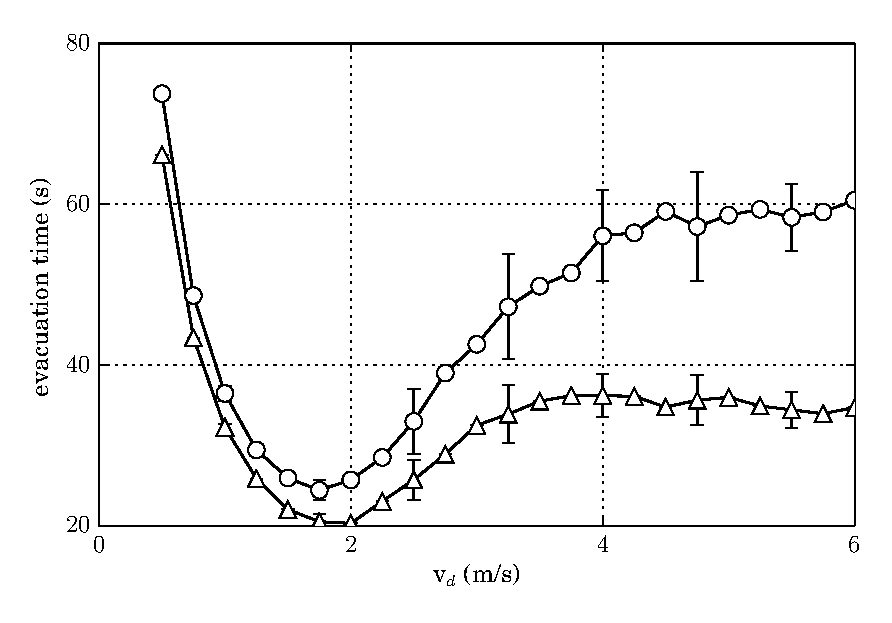
\includegraphics[scale=0.8]{figuras/fis_g.eps}
    \caption[width=5cm]{Tiempo de evacuación para 160 individuos (segundos) vs. la velocidad de deseo de los peatones (m/s). Two doors were available for leaving the room (see text for details). Los valores medios fueron computados para 30 procesos de evacuación. El ancho de cada puerta era $L=1,2$~m. Se muestran dos situaciones:  $\bigtriangleup$ corresponde a separación nula entre puertas, es decir, una única puerta de ancho  $2L$. $\bigcirc$ corresponde a una separación entre puertas de 1~m.}
    \label{fis_g}
\end{figure}

El tiempo de evacuación para puertas separadas siempre está por encima del tiempo que demora evacuar con una única puerta (\emph{i.e.} gap nulo). Para $v_d=6\,$m/s, una única salida reduce el tiempo de evacuación a la mitad con respecto al tiempo que demanda la configuración con $g=1\,$m. Otras distancias de separación (no exhibidas) muestran el mismo comportamiento que el de la figura \ref{fis_g}.\\

Puede decirse que aun dejando fijo el tamaño total de la abertura, separar este ancho en dos salidas simétricas puede afectar significativamente el rendimiento de la evacuación.

\subsection{Tiempo de evacuación}

En esta subsección se presentan los resultados de las mediciones de tiempo de evacuación en función de gap.
El tiempo de evacuación se define como el lapso que tarda una determinada cantidad de individuos ($\ge70\%$ de la cantidad inicial) en evacuar el recinto. \\

En la figura \ref{gap_vste_225_v4} se muestra la relación entre el tiempo de evacución y el gap para un recinto con 225 individuos con una velocidad de deseo de 4~m/s. Puede verse que el tiempo de evacuación aumenta mucho para gaps chicos hasta alcanzar el máximo en $g=1,5$~m. Para $g>1,5$~m, la pendiente de la curva se hace menor; el tiempo de evacuación disminuye a medida que aumenta el valor de $g$. 
Es decir, existe un gap crítico ($g_c$) para el cual cambia la pendiente de la curva.

\begin{figure}[H]
    \centering
    \includegraphics[scale=0.8]{figuras/gap_vste_225_v4_big.eps}
    \caption[width=5cm]{Gráfico de tiempo de evacuación en función del gap. El recinto es de $20\times 20$~(m) con 225 individuos y dos puertas, cada una tiene un ancho de $L=1,2$~m. La gráfica corresponde al promedio de treinta iteraciones. La velocidad deseada del individuo fue de $v_d=4$~m/s. Cada simulación termina cuando evacúan 160 individuos.}
    \label{gap_vste_225_v4}
\end{figure}

%\begin{figure}[H]
%    \centering
%    \includegraphics[height=5.5cm]{figuras/gap_vste_961_v4.eps}
%    \caption[width=5cm]{Gráfico de tiempo de evacuación en función del gap. El recinto es de $40\times 40$~(m) con 961 individuos y dos puertas, cada una tiene un ancho de $L=1,2$~m. La gráfica corresponde al promedio de treinta iteraciones. La velocidad deseada del individuo fue de $v_d=4$~m/s. Cada simulación termina cuando evacúan 864 individuos.}
%    \label{sintesis}
%\end{figure}

En el gráfico izquierdo de la figura \ref{gap_vste_vel_n} se muestra el tiempo de evacuación por individuo ($te/N$) en funcion de la distancia de separación de las puertas (gap). Se presentan tres curvas, cada una de ellas para recintos con diferente número de individuos: 961 (cuadrados), 584 (triángulos) y 225 (círculos). En todos los casos la pendiente de la curva cambia aproximadamente en $g=1,5$~m, por lo que el $g_c$ no depende del número de individuos. 
El tiempo de evacuación por individuo depende de N. A mayor cantidad de individuos mayor es $te/N$ para todo gap. 
Si bien en los tres casos la pendiente cambia luego del gap crítico, puede verse que para sistemas con 225 individuos la pendiente se hace ligeramente negativa mientras que para el resto la pendiente es prácticamente nula. \\
El gráfico de la derecha muestra el tiempo de evacuación en función del gap para recintos con 225 individuos. La curva con cuadrados corresponde a sistemas de individuos con velocidad de deseo $v_d=8$~m/s, la curva de círculos es para sistemas individuos con $v_d=4$~m/s. Ambas tienen igual valor de $g_c$, pero la curva correspondiente a $8~m/s$ no pasa a tener derivada negativa luego del $g_c$. Por lo tanto, el comportamiento para sistamas con individuos más apurados (8~m/s) es semejante al de sistemas con muchos individuos (961). \\
Cabe destacar que el tamaño de $g_c$ corresponde al ancho de dos individuos. Esto hace suponer que cuando el espacio entre puertas es suficientemente grande para que entren dos personas, la dinámica entra en un régimen diferente. 

\begin{figure}[H]
    \centering
    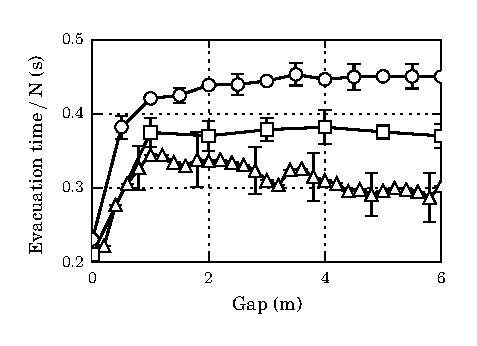
\includegraphics[scale=1]{figuras/fig1_version0.eps}
    \includegraphics[scale=1]{figuras/gap_vste_225_v4_v8.eps}
    \caption[width=5cm]{Gráfico de tiempo de evacuación en función del gap para recintos de $20\times 20$~(m) (círculos), $30\times 30$~(m) (triángulos) y $40\times 40$~(m) (cuadrados) con 225, 580 y 961 individuos respectivamente. Todos los recintos tienen dos puertas, cada una de ancho $L=1,2$~m. Las gráficas corresponden al promedio de treinta iteraciones. Para todos los casos, la velocidad deseada del individuo fue de $v_d=4$~m/s. Cada simulación termina cuando evacúan 160, 529 y 961 individuos respectivamente.
    Derecha: Gráfico de tiempo de evacuación en función del gap. El recinto es de $20\times 20$~(m) con 225 individuos y dos puertas, cada una tiene un ancho de $L=1,2$~m. La gráfica corresponde al promedio de treinta iteraciones. Las velocidades de deseo de los individuos es de $v_d=4$~m/s (círculos) y $v_d=8$~m/s (cuadrados). Cada simulación termina cuando evacúan 160 individuos.}
    \label{gap_vste_vel_n}
\end{figure}


%\begin{figure}[H]
%    \centering
%    \includegraphics[height=5.5cm]{figuras/gap_vste_v4_v8.png}
%    \caption[width=5cm]{Gráfico de tiempo de evacuación en función del gap. El recinto es de $20\times 20$~(m) con 225 individuos y dos puertas, cada una tiene un ancho de $L=1,2$~m. La gráfica corresponde al promedio de treinta iteraciones. Las velocidades de deseo de los individuos es de $v_d=4$~m/s y $v_d=8$~m/s. Cada simulación termina cuando evacúan 160 individuos.}
%    \label{sintesis}
%\end{figure}


\subsection{Blocking clusters}

En esta subsección se compararán las diferencias en la probabilidad de formar clusters de bloqueo grandes (que abarcan ambas puertas) y chicos (abarcan solo una puerta). También se muestra cómo esta probabilidad depende de la cantidad de indviduos y la velocidad de deseo.\\
Un sistema de 225 individuos con $v_d=4$~m/s manifiesta, en la figura \ref{proba_vsgap_v4_big_small}, que la probabilidad de formar big blocking clusters (círculos) decae con la separación de las puertas. Es decir, cuanto más lejos están las puertas es más dificil lograr una unión de individuos que vaya de un extremo al otro.
Por otro lado, la probabilidad de formar clusters de bloqueo pequeños (bloqueos de una única puerta) tiene una forma funcional que alcanza el máximo en el $g_c$ y luego desciende. Este comportamiento es similar al de tiempo de evacuación en función del gap.\\
El tamaño del gap critico equivale al ancho de dos individuos. Este tamaño favorece la formación de dos blocking clusters (uno para cada puerta). Esto genera un aumento de los bloqueos que se manifiesta en un incremento del tiempo de evacuación. 


\begin{figure}[H]
    \centering
    \includegraphics[scale=0.8]{figuras/proba_vsgap_v4_big_small.eps}
    \caption[width=5cm]{Probabilidad de formar big y small blocking clusters (bloqueos de dos y una puerta respectivamente) en función del gap. El recinto es de $20\times 20$~(m) con 225 individuos y dos puertas, cada una tiene un ancho de $L=1,2$~m. Las gráficas corresponden al promedio de treinta iteraciones diferentes. La velocidad de deseo es de $v_d=4$~m/s. Cada simulación termina cuando evacúan 160 individuos.}
    \label{proba_vsgap_v4_big_small}
\end{figure}

La probabilidad de formar clusters de bloqueo esta sujeta al número de individuos y la velocidad de deseo. Esto puede verse en la figura \ref{proba_vsgap_all} donde la curva con triángulos representa la probabilidad de formar blocking clusters para un recinto con 961 individuos, la curva que esta debajo (cadrados) es para un sistema con 225 individuos con velocidad de deseo $v_d=6$~m/s y la curva con círculos corresponde a $v_d=4$~m/s y 225 peatones. Incrementar N o $V_d$ produce un aumento de la probabilidad de formar clusters de bloqueo. Es decir, si los individuos estan apurados o si el tamaño de la multitud es grande, aumentan los lapsos de tiempo en los cuales las puertas están bloqueadas.  

\begin{figure}[H]
    \centering
    \includegraphics[scale=0.8]{figuras/proba_vsgap_all_big.eps}
    \caption[width=5cm]{Probabilidad de formar small blocking clusters (bloqueos de una sola puerta) en función del gap, para un recinto $20\times 20$~(m) con 225 individuos a $v_d=4$~m/s y $v_d=6$~m/s. Lo mismo para un recinto de $40\times 40$~(m) con 961 individuos a $v_d=4$~m/s. Ambos recintos poseén dos puertas, cada una tiene un ancho de $L=1,2$~m. Las gráficas corresponden al promedio de treinta iteraciones diferentes. Las simulación terminan cuando evacúan 160 individuos y 864 respectivamente.}
    \label{proba_vsgap_all}
\end{figure}

%\begin{figure}[H]
%    \centering
%    \includegraphics[height=5.5cm]{figuras/proba_vsgap_small_225p_v4.png}
%    \caption[width=5cm]{Probabilidad de formar small blocking clusters (bloqueos de una sola puerta) en función del gap. El recinto es de $20\times 20$~(m) con 225 individuos y dos puertas, cada una tiene un ancho de $L=1,2$~m. La gráfica corresponde al promedio de treinta iteraciones. La velocidad de deseo es de $v_d=4$~m/s. Cada simulación termina cuando evacúan 160 individuos.}
%    \label{sintesis}
%\end{figure}

%\begin{figure}[H]
%    \centering
%    \includegraphics[height=5.5cm]{figuras/proba_vsgap_small_961p_v4.png}
%    \caption[width=5cm]{Probabilidad de formar small blocking clusters (bloqueos de una sola puerta) en función del gap. El recinto es de $40\times 40$~(m) con 961 individuos y dos puertas, cada una tiene un ancho de $L=1,2$~m. La gráfica corresponde al promedio de treinta iteraciones diferentes. La velocidad de deseo es de $v_d=4$~m/s. Cada simulación termina cuando evacúan 864 individuos.}
%    \label{sintesis}
%\end{figure}



\subsection{Presión}

En esta subsección se describirán los diagramas de isobaras para recintos con dos puertas separadas por un gap. 
Cuando la separación es nula (gap cero) se recupera una distribución de presión similar a las distribuciones de la sección anterior. La presión máxima se da en los costados ya que en el medio se forma un canal por donde la gente puede transitar (figura \ref{presion_225p_g0}). Se tiene simetría de reflexión con respecto al eje $y=10$~m. 
\begin{figure}[H]
    \centering
    \includegraphics[scale=1]{figuras/press_225p_v4_g0.eps}
    \caption[width=5cm]{Isobaras cercanas a la puerta; la escala a la derecha está expresada en [PV]=N.m. La salida está centrada en la posición $x=20$~m e $y=10$~m, son dos puertas de ancho $L=1,2$~m con $g=0$~m. El recinto es de $20\times 20$~(m) con 225 individuos. La gráfica corresponde a valores medios a lo largo de 30 procesos de evacuación. Se usó un grillado de 1m$^2$ para promediar el campo de presiones (PV). La velocidad deseada de los individuos fue de $v_d=4$~m/s.}
    \label{presion_225p_g0}
\end{figure}

Cuando la separación entre puertas equivale al gap crítico $g=1,5$~m, la zona de más alta presión se extiende en superficie. Si $g=5$~m los focos de máxima presión se separan ya que a esta distancia los bulks están suficientemente lejos como para que las interacciones entre éstos sean chicas. Este fenómeno se muestra en las figuras de \ref{presion_225p_g1_5_y_5}. Puede verse que cuando el gap es grande no existen zonas de presión alta ($>$8000 N.m). Separar las puertas una distancia considerable produce una disminución general de la presión.    

\begin{figure}[H]
    \centering
    \includegraphics[scale=1]{figuras/isobaras_g1_5.eps}
        \includegraphics[scale=1]{figuras/isobaras_g5.eps}	
    \caption[width=5cm]{Isobaras cercanas a la puerta; la escala a la derecha está expresada en [PV]=N.m. La salida consta de dos puertas de ancho $L=1,2$~m separadas entre si por una distancia de $g=1,5$~m y $g=5$~m (figuras de izquierda y derecha respectivamente), puertas centrdas en $x=20$~m e $y=11,35$~m y $x=20$~m e $y=8,65$~m (izquierda) y $x=20$~m e $y=12,5$~m y $x=20$~m e $y=7,5$~m (derecha) . El recinto es de $20\times 20$~(m) con 225 individuos. Las gráficas corresponde a valores medios a lo largo de 30 procesos de evacuación. Se usó un grillado de 1m$^2$ para promediar el campo de presiones (PV). La velocidad deseada de los individuos fue de $v_d=4$~m/s.}
    \label{presion_225p_g1_5_y_5}
\end{figure}

%\begin{figure}[H]
%    \centering
%    \includegraphics[scale=1]{figuras/isobaras_g5.eps}			\caption[width=5cm]{Isobaras cercanas a la puerta; la escala a la derecha está expresada en [PV]=N.m. La salida consta de dos puertas de ancho $L=1,2$~m separadas entre si por una distancia de $g=1,5$~m, centrdas en $x=20$~m e $y=12,5$~m y $x=20$~m e $y=7,5$~m. El recinto es de $20\times 20$~(m) con 225 individuos. La gráfica corresponde a valores medios a lo largo de 30 procesos de evacuación. Se usó un grillado de 1m$^2$ para promediar el campo de presiones (PV). La velocidad deseada de los individuos fue de $v_d=4$~m/s.}
%    \label{presion_225p_g5}
%\end{figure}


En esta sección se discutieron los resultados para recintos con dos puertas separadas por un gap. Se obtuvo que el efecto "faster is slower" vale para distintos grados de separación. Las curvas de tiempo de evacuacón presentan un cambio de derivada  luego del gap crítico ($g_c$=1,5~m). El comportamiento cualitativo de la probabilidad de formar blocking clusters es similar al del tiempo de evacuación. Por lo tanto el bloqueo de cada una de las puertas es un factor determinante en la evacuación. En cuanto a la presión, si las puertas están suficientemente alejadas se produce una disminución general de la misma debido a la formación de bulks con menos individuos. 


%\subsection{Comportamiento asintótico}


